\documentclass[a4paper]{instrumentacao}

\usepackage{listings}
\usepackage{etoolbox}
\usepackage{graphicx}

\newtoggle{attachments}
\togglefalse{attachments}

\graphicspath{
	{../Resources/Images/}
	{../Resources/Mathematica/images/}
	{../Resources/MATLAB/images/}
}

%todo colocar um titulo "criativo"
\title{Sobre sensores Pt100 e NTC}
\author{Rogiel Sulzbach \and Rodrigo de Castro Silveira \and Yi Chen Wu}
\startdate{11/04/2016}
\finishdate{09/05/2016}
\emails{
	\emailaddress{R.J.S.}{rogiel@rogiel.com},
	\emailaddress{R.C.S.}{csilveira.rodrigo@gmail.com} e
	\emailaddress{Y.C.}{yichenpoa@gmail.com}
}
\resume{}
\abstract{}
\keywords{}
\institute{Universidade Federal do Rio Grande do Sul, Departamento de Engenharia Elétrica, Curso de Engenharia Elétrica, Instrumentação A, Profs. Dr. Alexandre Balbinot e Dra. Léia Bagesteiro}

\headertext{Termometria}

\begin{document}
\maketitle


\chapter{Introdução}
A termometria é uma parte da termologia que estuda a temperatura e as formas pelas quais ela pode ser medida.  É uma das grandes áreas da Instrumentação e, sem dúvida, uma das mais importantes. O controle e monitoramento de temperatura é uma variável de grande valia em diversos sistemas, principalmente em processos industriais, onde a temperatura de fornos, por exemplo, devem ser cuidadosamente monitorados para que o produto não sofra avalias ou deformações na sua estrutura.

A temperatura é uma grandeza associada à energia cinética média das moléculas de um corpo. Quando a temperatura de um corpo muda, algumas propriedades desse corpo se modificam. Por exemplo:

\begin{itemize}
	\item Quando se aquece um líquido, o volume deste líquido aumenta.
	\item Quando se aquece uma barra de metal, o comprimento desta barra aumenta.
	\item Quando se aquece um fio elétrico, a resistência deste fio elétrico aumenta.
	\item Quando se aquece um gás confinado, a pressão deste gás confinado aumenta.
\end{itemize}

Estas propriedades podem ser usadas para criar um instrumento capaz de medir a temperatura de um corpo, colocando um desses tipos de material em contato com o corpo.

\chapter{Metodologia Experimental}

Nestes experimentos de laboratório foi utilizado o software Wolfram Mathematica 10.4.0 da Wolfram Research, Inc. para realizar todos os cálculos no computador utilizando precisão do tipo MachinePrecision\cite{mathematica-numerial-precision} onde a precisão dos números de ponto flutuante respeitam os critérios impostos pelo processador (64 bits, precisão dupla) que implementam o padrão IEEE de ponto flutuante, possuem um "Épsilon de Máquina", o menor valor que somado a 1 retorna um valor diferente de 1, isto é, não causa arredondamento \cite{wikipedia-epsilon}, de $2^{-52}$, ou seja, na ordem de $10^{-16}$ e podem, portanto, serem desprezados perante a resolução de todos os outros instrumentos instrumentos utilizados no experimento. Adicionalmente, quando possível, os cálculos foram realizados de forma simbólica com substituição numérica no final. Os scripts utilizados para cálculo estão anexados ao fim do documento, na Página \pageref{ch:attachments}.

\section{Sensor de temperatura baseado em Pt100}
\label{ch:pt100}

\subsection{Calibração do sensor Pt100}
Pt100 é o nome dado a um tipo de termoresistor composto de Platina cuja variação de resistência elétrica é associada à variação de temperatura de forma linear. Outra caraterística importante é que a resistência elétrica nominal a $0ºC$ é de $100 \Omega$. Sendo um sensor linear, faz com que a criação de um termômetro eletrônico seja mais simples do que outros sensores não lineares ou de utilização mais complexa, embora a inércia térmica do sensor não permita que sejam feitas medidas em frequências elevadas como os sensores do tipo termopares permitem.

A função de transferência teórica do Pt100 é dada pela Equação \ref{eq:pt100} \cite{livro-texto}:

\begin{equation}
	R(T) = R_0 \left[1 + \alpha\left(T - T_0\right)\right]
	\label{eq:pt100}
\end{equation}

\noindent
onde $R(T)$ é a resistência elétrica em $\Omega$ do Pt100 para uma dada temperatura $T$ em $ºC$, $\alpha$ é uma constante dependente de características de construção do Pt100, $R_0$ é a resistência de referência em $\Omega$ (tipicamente $100 \Omega$ para o Pt100) e $T_0$ é a temperatura de referência em $ºC$ do termoresistor (tipicamente $0ºC$ para o Pt100).

Pode-se ainda isolar o coeficiente de temperatura $\alpha$ da Equação \ref{eq:pt100}:

\begin{equation}
	\alpha=\frac{R-R_0}{R_0(T-T_0)}
	\label{eq:pt100-alpha}
\end{equation}

A sensibilidade do sensor  de temperatura é, por definição, a razão da variável de saída pela variável de entrada \cite{livro-texto}. Assim, é necessário derivar a Equação \ref{eq:pt100} e calcular $S$:

\begin{equation}
	S_{Pt100}=\frac{dR}{dT}=\frac{d[R_0(1+\alpha(T-T_0))]}{dT}=\alpha R_0
	\label{eq:pt100-sensibilidade}
\end{equation}

Para estimar a função de transferência experimental do termoresistor, projetou-se um experimento onde foram feitas 2 medidas de forma aleatória para temperaturas de $18ºC$ até $78ºC$, graduadas em $2ºC$ cada. Na Figura \ref{fig:pt100-esquematico} está apresentado um desenho simplificado da configuração utilizada no experimento.

\begin{figure}[H]
\center
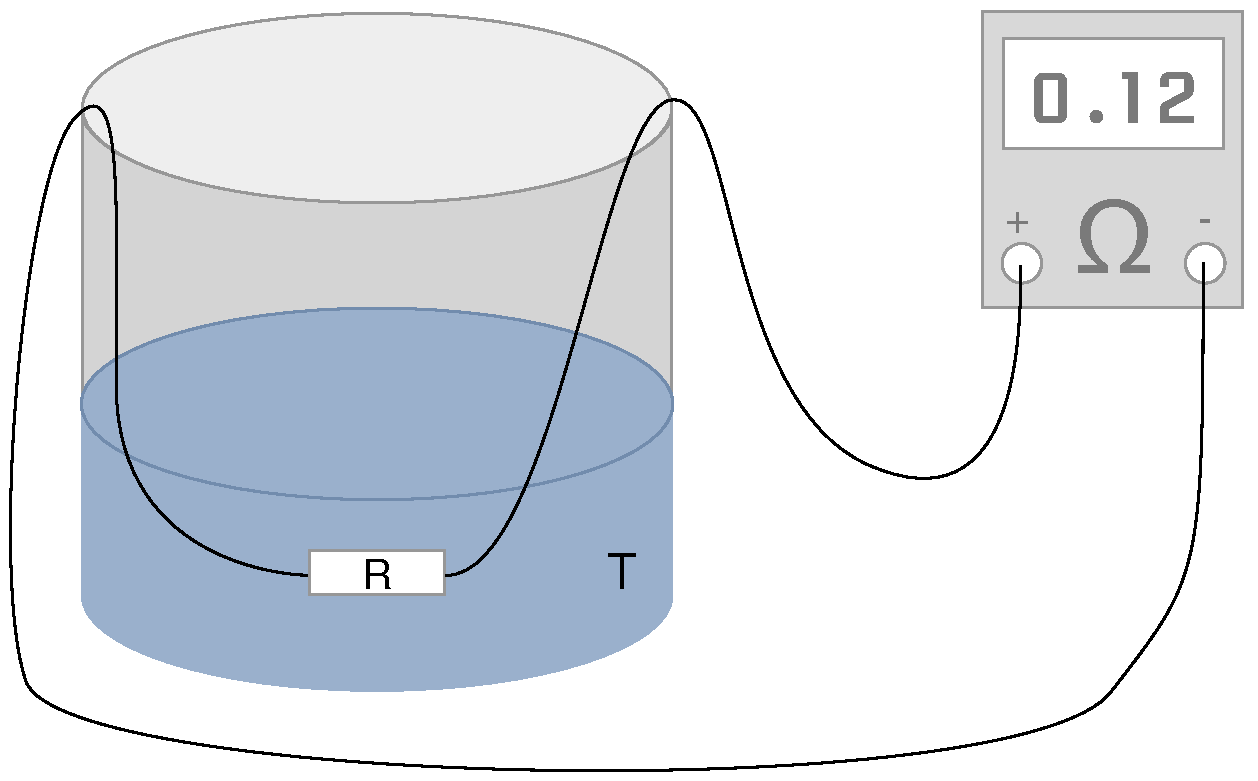
\includegraphics[width=\textwidth]{Bequer.pdf}
\caption{Desenho esquemático do experimento -- dentro de um béquer é colocada água com temperatura variando de $18ºC$ à $78ºC$ e mede-se a resistência elétrica correspondente do termoresistor.}
\label{fig:pt100-esquematico}
\end{figure}

\noindent
onde $R$ é um termoresistor Pt100, $T$ é a temperatura da água dentro do copo de Béquer, e o instrumento $\Omega$ é um ohmímetro.

As medidas foram feitas de forma aleatória e com 2 repetições por célula. Após a extração dos resultados, fez-se o ajuste de curvas e obteve-se a função de transferência experimental do termoresistor.

Com o copo de Béquer preenchido com água até a metade para que o processo de aquecimento não levasse muito tempo e nem que fosse necessário aguardar o aquecimento de um grande volume de água nem resfriar o mesmo. Uma vez que a temperatura da agua estivesse ajustada na temperatura desejada, o valor de resistência elétrica correspondente mostrado no multímetro foi anotado.

Para fazer o ajuste de temperatura da água até a temperatura de interesse foram utilizadas 2 práticas: o uso de um aquecedor elétrico para elevar a temperatura e adição de água gelada para abaixar a temperatura. Isto é, caso a temperatura de interesse estivesse acima da temperatura atual da água, um aquecedor elétrico foi utilizado para elevar a temperatura e comparar utilizando um termômetro comercial de referência e caso a temperatura de interesse estivesse abaixo da temperatura atual da água, uma pequena porção de água gelada foi adicionada ao copo até que a temperatura de desejo fosse obtida.

O termômetro comercial utilizado não possuía identificação com nome do fabricante mas informa que tem resolução de 0.1ºC dentro do intervalo de interesse com incerteza de 1ºC. Acredita-se (este fator não foi testado) que o termômetro faz uso de uma média móvel com janela entre 20 e 30 segundos devido ao tempo de resposta perceptível do termômetro durante a execução do experimento. Devido a isto, aguardava-se para que o valor mostrado no \textit{display} da referência estivesse, por, pelo menos, 10 segundos num valor estável.

Enquanto o aquecedor estava ligado ou logo após a adição de água gelada, com uma colher de plástico, a água era agitada para que a temperatura fosse homogeneizada por todo volume. Também foi tomado o devido cuidado para que o nem sensor nem o termômetro de referência ficassem muito próximos do aquecedor que poderia causar danos à eles ou provocar erros sistemáticos de medida devido ao super aquecimento interno nos componentes que não pudessem ser facilmente dissipados na duração do experimento.

Como \textit{ohmímetro} foi utilizado um multímetro digital da Minipa, modelo ET-2082b, que possui as especificações de precisão conforme é apresentada na Tabela \ref{tab:precisao-multimetro}. 

\begin{table}[H]
\centering
\caption{Especificações de Precisão do multímetro digital Minipa ET-2082b - Escala de resistência elétrica}
\label{tab:precisao-multimetro}
\begin{tabular}{|c|c|c|}
\hline
\textbf{Faixa} & \textbf{Precisão}                 & \textbf{Resolução} \\ \hline
200 $\Omega$           & $\pm$ (0.8\%+5D)                  & 0.1 $\Omega$                 \\ \hline
2 k$\Omega$             & \multirow{4}{*}{$\pm$ (0.8\%+3D)} & 1 $\Omega$                   \\ \cline{1-1} \cline{3-3} 
20 k$\Omega$            &                                   & 10 $\Omega$                  \\ \cline{1-1} \cline{3-3} 
200 k$\Omega$           &                                   & 100 $\Omega$                 \\ \cline{1-1} \cline{3-3} 
2 M$\Omega$             &                                   & 1 k$\Omega$                 \\ \hline
20 M$\Omega$            & $\pm$ (1.0\%+15D)                 & 10 k$\Omega$                \\ \hline
2000 M$\Omega$          & $\pm$ {[}5\%(Leit.-10D)+20D{]}    & 1 M$\Omega$                 \\ \hline
\end{tabular}
\end{table}


\todo{resto do experimento do pt100}

\section{Sensor de temperatura baseado em NTC}
\label{ch:ntc}
\subsection{Calibração do sensor NTC}
O NTC (\textit{Negative Temperature Coefficient}) é um termoresistor, não-linear cujo coeficiente de temperatura é negativo e, portanto, sua resistência elétrica decai à medida que a temperatura se eleva.

Analogamente ao sensor de temperatura baseado em Pt100 (Página \pageref{ch:pt100}), para que seja possível a construção de um termômetro utilizando um sensor do tipo NTC, é necessário que primeiramente seja levantada a função de transferência do componente para que seja possível utilizá-la na cadeia de medidas do termômetro.

A função de transferência teórica do NTC é dada pela Equação \ref{eq:ntc} \cite{livro-texto}.

\begin{equation}
	\large
	R(T) \approxeq R_0 e^{\beta\left(\frac{1}{T} - \frac{1}{T_0}\right)}
	\label{eq:ntc}
\end{equation}

\noindent
onde $R(T)$ é a resistência elétrica em $\Omega$ do NTC para uma dada temperatura $T$ em $K$, $\beta$ é uma constante dependente do material e características de construção do NTC, $R_0$ é a resistência de referência em $\Omega$ e $T_0$ é a temperatura de referência do termoresistor em $K$.

Para estimar a função de transferência experimental do NTC, projetou-se um experimento onde foram feitas 2 medidas de forma aleatória para temperaturas de $18ºC$ até $78ºC$, graduadas em $2ºC$ cada. Na Figura \ref{fig:ntc-esquematico} está apresentado um desenho simplificado da configuração utilizada no experimento.

\begin{figure}[H]
\center
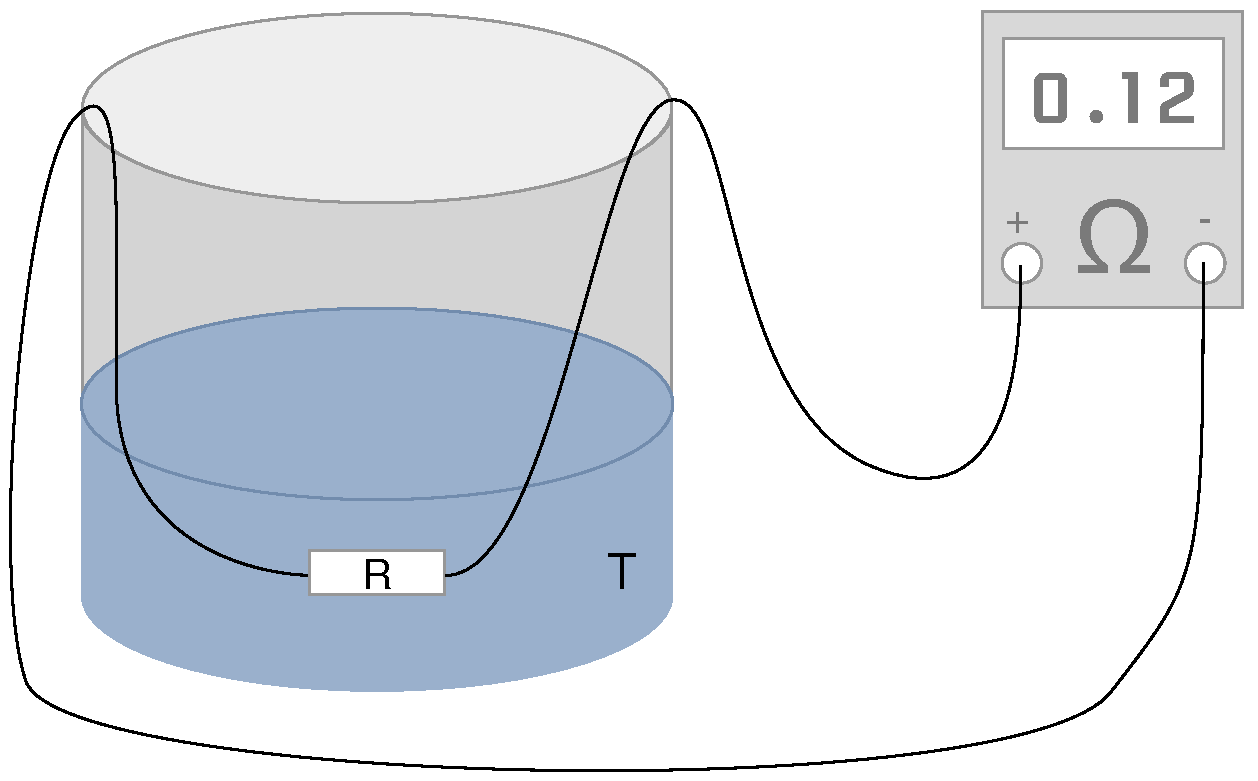
\includegraphics[width=\textwidth]{Bequer.pdf}
\caption{Desenho esquemático do experimento -- dentro de um béquer é colocada água com temperatura variando de $18ºC$ à $78ºC$ e mede-se a resistência elétrica correspondente do NTC.}
\label{fig:ntc-esquematico}
\end{figure}

\noindent
onde $R$ é um termoresistor NTC, $T$ é a temperatura da água dentro do copo de Béquer em $K$, e o instrumento $\Omega$ é um ohmímetro.

As medidas foram feitas de forma aleatória e com 2 repetições por célula. Após a extração dos resultados, fez-se o ajuste de curvas e obteve-se a função de transferência experimental do termoresistor.

A cadeia de medidas deste experimento é dada pela Figura \ref{fig:ntc-cadeia-medidas}:

\begin{figure}[H]
\center
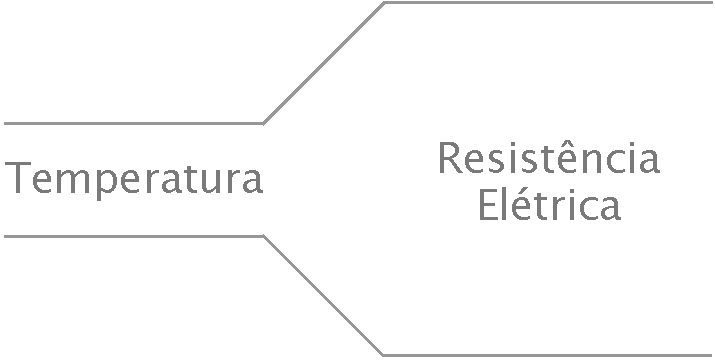
\includegraphics[width=0.7\textwidth]{CadeiaMedidas.pdf}
\caption{Cadeia de medidas para o sensor NTC}
\label{fig:ntc-cadeia-medidas}
\end{figure}

\noindent
onde a entrada é dada em temperatura (ºC) e a saída é dada em resistência elétrica ($\Omega$).




\chapter{Resultados e Discussões}
\section{Sensor de temperatura baseado em Pt100}
Com base na metodologia apresentada na seção \ref{ch:pt100} da Metodologia Experimental, foram levantadas os valores da resistência elétrica para o sensor Pt100, na faixa especificada, com 2 amostras por temperatura. Os resultados são observados da Tabela \ref{tab:amostras-pt100}, que mostra também uma coluna com o valor médio para cada temperatura, com base nas duas medições. O multímetro foi utilizado na escala de resistência elétrica, para a faixa de 200 $\Omega$, e possui precisão e resolução conforme apresenta da Tabela \ref{tab:precisao-multimetro}.

\begin{table}[]
\centering
\caption{Amostras de medidas de resistência elétrica do Pt100 - Temperatura 18ºC a 76ºC}
\label{tab:amostras-pt100}
\begin{tabular}{|c|c|c|c|}
\hline
\textbf{Temp. ($ºC$)} & \textbf{Medida 1 ($\Omega$)} & \textbf{Medida 2 ($\Omega$)} & \textbf{Média ($\Omega$)} \\ \hline
18                  & 106,8                 & 107,0                 & 106,9          \\ \hline
20                  & 108,4                 & 108,1                 & 108,3          \\ \hline
22                  & 109,0                 & 108,9                 & 109,0          \\ \hline
24                  & 109,4                 & 109,6                 & 109,5          \\ \hline
26                  & 110,2                 & 110,4                 & 110,3          \\ \hline
28                  & 111,0                 & 111,1                 & 111,1          \\ \hline
30                  & 111,9                 & 111,9                 & 111,9          \\ \hline
32                  & 112,7                 & 112,5                 & 112,6          \\ \hline
34                  & 113,3                 & 113,5                 & 113,4          \\ \hline
36                  & 114,1                 & 114,2                 & 114,2          \\ \hline
38                  & 115,0                 & 114,9                 & 115,0          \\ \hline
40                  & 115,7                 & 115,8                 & 115,8          \\ \hline
42                  & 116,6                 & 116,4                 & 116,5          \\ \hline
44                  & 117,3                 & 117,4                 & 117,4          \\ \hline
46                  & 117,9                 & 118,1                 & 118,0          \\ \hline
48                  & 118,8                 & 118,8                 & 118,8          \\ \hline
50                  & 119,5                 & 119,7                 & 119,6          \\ \hline
52                  & 120,8                 & 120,6                 & 120,7          \\ \hline
54                  & 121,1                 & 121,0                 & 121,1          \\ \hline
56                  & 121,7                 & 121,7                 & 121,7          \\ \hline
58                  & 122,7                 & 123,0                 & 122,9          \\ \hline
60                  & 123,4                 & 123,3                 & 123,4          \\ \hline
62                  & 124,4                 & 124,1                 & 124,3          \\ \hline
64                  & 124,8                 & 124,8                 & 124,8          \\ \hline
66                  & 125,4                 & 125,5                 & 125,5          \\ \hline
68                  & 126,3                 & 126,3                 & 126,3          \\ \hline
70                  & 127,0                 & 126,8                 & 126,9          \\ \hline
72                  & 128,0                 & 127,9                 & 128,0          \\ \hline
74                  & 128,6                 & 128,5                 & 128,6          \\ \hline
76                  & 129,1                 & 129,3                 & 129,2          \\ \hline
\end{tabular}
\end{table}

A Figura \ref{fig:pt100-amostras} \todo{verificar se fica esse ou faz outro gráfico no Mathematica} mostra os pontos de temperatura verificados, bem como a curva ajustada para os valores obtidos.

\begin{figure}[H]
\center
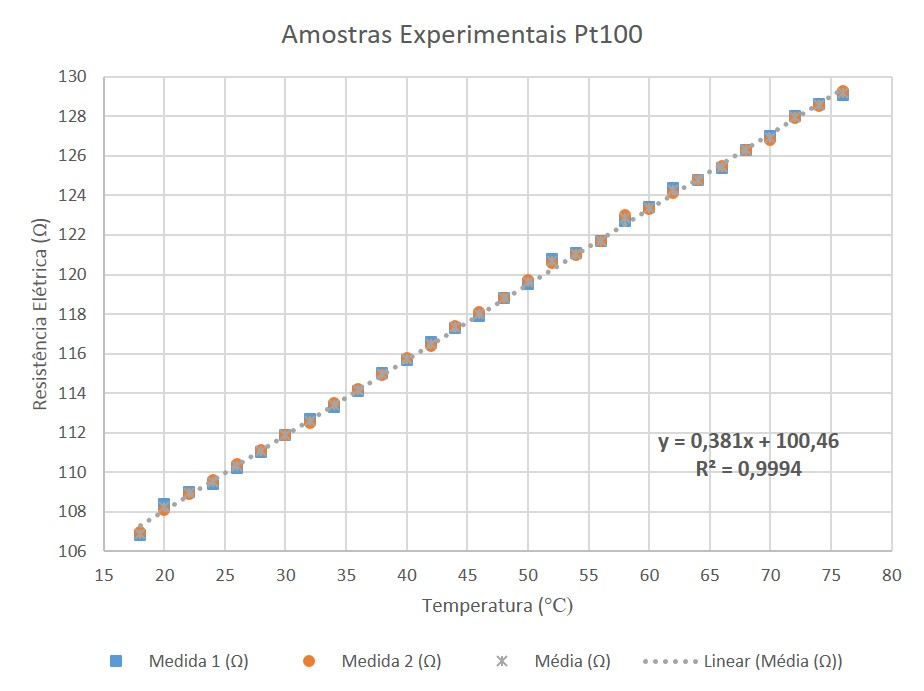
\includegraphics[width=0.7\textwidth]{pt100_puro.jpg}
\caption{Gráfico das amostras experimentais apresentando a variação da resistência elétrica em função da variação da temperatura da água.}
\label{fig:pt100-amostras}
\end{figure}

A regressão linear, com base nos valores da média das amostras obtidas, apresentou como função de transferência experimental os seguintes resultados:

\begin{equation}
	R(T) = 0.381*T + 100.46
	\label{eq:pt100-reg}
\end{equation}
\begin{equation}
	R^2=0.9994
	\label{eq:pt100-reg-r2}
\end{equation}

\noindent
onde $R(T)$ é a resistência elétrica, em $\Omega$, do sensor Pt100, e $T$ é a temperatura, em $ºC$, percebida pelo sensor.

A Equação \ref{eq:pt100-reg-r2} apresenta o valor do coeficiente de linearidade, significando que 99,94\% da variável dependente consegue ser explicada pelos regressores presentes no modelo.

Com base na Equação \ref{eq:pt100-alpha} pode-se facilmente encontrar o valor do coeficiente de temperatura $\alpha$. Também é possível notar, igualando as Equações \ref{eq:pt100} e \ref{eq:pt100-reg}, que:

\begin{eqnarray}
	R_0 &=& 100.46 [\Omega]\\
	\alpha R_0 &=& 0.381 [\frac{\Omega}{ºC}] \label{eq:pt100-alpha-valor}
\end{eqnarray}

De onde se pode extrair o valor de $\alpha$:
\begin{eqnarray}
	\alpha &=& \frac{0.381}{R_0} \\
	       &=& 0.00379 [\frac{\Omega}{\Omega ºC}]
\end{eqnarray}

O valor de $\alpha$ encontrado experimentalmente é compatível com o valor tabelado pela Norma \textit{IEC 751}, que é de 0.00385 $\frac{\Omega}{\Omega ºC}$ para \textit{RTDs} de Platina, que é o caso do Pt100.

Nota-se ainda que a Equação \ref{eq:pt100-alpha-valor} apresenta o valor da sensibilidade $S_{Pt100}$ do sensor.

\section{Sensor de temperatura baseado em NTC}

\chapter{Conclusões}

\todo{lembrar as escalas dos multímetros}

\newpage
\begin{thebibliography}{9}
\bibitem{mathematica-numerial-precision} \url{https://reference.wolfram.com/language/tutorial/NumericalPrecision.html}, acessado em 26 de abril de 2016
\bibitem{wikipedia-epsilon} \url{https://en.wikipedia.org/wiki/Machine_epsilon}, acessado em 26 de abril de 2016
\bibitem{livro-texto}  Balbinot, Alexandre; Brusamarello, Valner J., Instrumentação e Fundamentos de Medida - Vol.1 - 2ª Ed. Rio de Janeiro: LTC, 2014.


%\bibitem{datasheet-lm7905} Datasheet oferecido pelo fabricante do regulador de tensão LM7905PI, disponível em \url{http://www.datasheetlib.com/datasheet/190159/kia7905pi_kec-korea-electronics-corporation.html}.

%\bibitem{datasheet-lm7805} Datasheet oferecido pelo fabricante do regulador de tensão LM7805CV, disponível em \url{http://www.datasheetlib.com/datasheet/221840/l7805cv_stmicroelectronics.html}.

%\bibitem{datasheet-lm741} Datasheet oferecido pelo fabricante do amplificador operacional LM741, disponível em \url{http://www.datasheetlib.com/datasheet/818655/lm741_ti-texas-instruments.html}.




%\bibitem{ref1} Sobrenome, A.B.; Sobrenome, C.D. Title of the cited article. Journal Title 2007, 6, 100-110. 
%\bibitem{ref2} Balbinot, A.; Brusamarello, V.J.. Title of the cited article. Journal Title 2007, 6, 100-110. 
%\bibitem{ref3} Author, A.; Author, B. Title of the chapter. In Book Title, 2nd ed.; Editor, A., Editor, B., Eds.; Publisher: Publisher Location, Country, 2007; Volume 3, pp. 154-196.
%\bibitem{ref4} Author, A.; Author, B. Book Title, 3rd ed.; Publisher: Publisher Location, Country, 2008; 
%pp. 154-196.

\end{thebibliography}

\iftoggle{attachments}{
	\chapter*{Anexos}
	\label{ch:attachments}
	\section{Mathematica}
	\includenotebook{../Resources/Mathematica/Experimento 1-1.nb.pdf}{Pêndulo}{pendulo}
	\includenotebooksingle{../Resources/Mathematica/Incerteza potenciometro.nb}{Incerteza do potenciômetro}{incerteza-potenciometro}
	\includenotebooksingle{../Resources/Mathematica/Incertezas-Filtro.nb}{Incerteza do filtro}{incerteza-filtro}

	\section{MATLAB}
	\label{att:script-matlab}
	\lstinputlisting[
		language=MATLAB,
		numbers=left,
		caption={Script MATLAB para análise de frequência}
	]{../Resources/MATLAB/primeiro.m}
}

\end{document}
